
\chapter{Results}\label{chap:evaluation}
% \section{Prototyping/Evaluating the System}
% 5-7 pages
\lipsum[1]\todo{TODO}

This section describes the evaluation of the solution, by describing the environment setup, the pipeline deployment framework, the training data collection and labelling steps, the neural network implementation and training. Finally, the pose estimation algorithms and the pipeline are evaluated.

\section{Environment Setup}
    The design rationale main purpose was to allow for portability and plug-and-play behavior of pose estimation algorithms. We also attempt to minimize assumptions on poses or camera angles (frame information) and account for the natural variation of the cow teats (udder morphology, colors, light conditions, etc.). As proof of concept for the project the test environment that was set up consisted of an artificial cow at the ZHAW and a robotic arm as shown by Figure \ref{fig:cow_setup}.
    
    \begin{figure}[h]
        \centering
        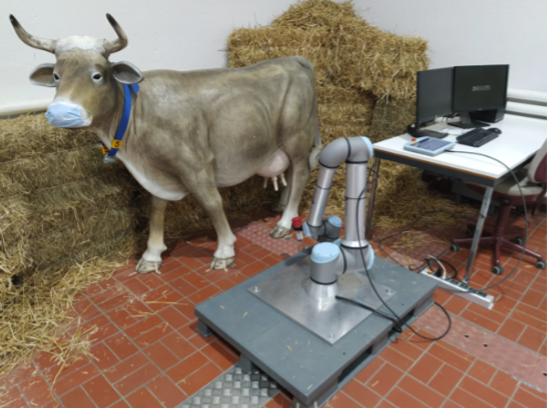
\includegraphics[width=0.65\textwidth]{images/cow_setup.png}
        \caption{A prototype of the Job Information dialog}
        \label{fig:cow_setup}
    \end{figure}
    The hardware setup for such an environment consisted of:
    \begin{itemize}
        \item \textbf{Blackbox PC:} where the Robot Operating System was running the pose estimation and the robot manipulation.
        \item \textbf{UR10e robot:} industrial robot used in machine tending, palletizing, and packaging (6 axis).
        \item \textbf{Arm Flange:} the flange at the end of the arm had the camera and the milking cup.
        \item \textbf{Dummy cow:} artificial cow model with fake teats to test the robotic attachment.
    \end{itemize}
   
    \begin{figure}[h]
        \centering
        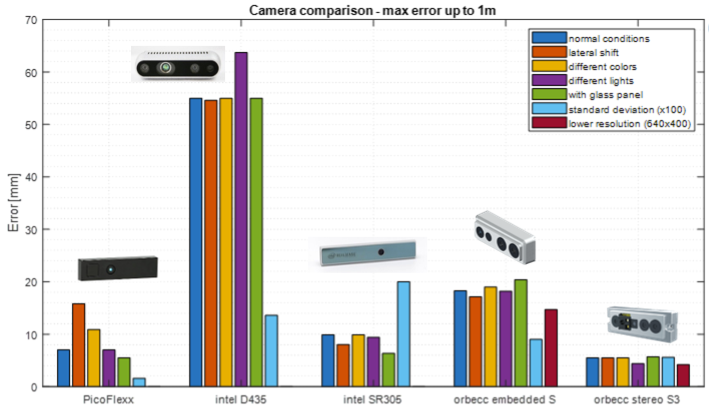
\includegraphics[width=0.8\textwidth]{images/camera_choice.png}
        \caption{Camera performance comparison.}
        \label{fig:camera_choice}
    \end{figure}
    
    The camera evaluation was done considering light conditions, shifting, object colors, a glass panel and lower resolutions: Figure \ref{fig:camera_choice} shows the performance of different camera models (for the detail on the camera names and manufacturers look at Appendix \ref{appendix:camera_choice}).
\section{Pipeline Deployment}
The deployment of the components was done using docker compose files to leverage the capabilities of microservices, where every component used behaves as a separate component in the application. The benefit gotten out of microservices is that they are small in size, bounded by their context, independently developed and deployable and they allow for message-based communication%todo ADD REF
. 

The set of libraries and tools used for building the robot application for pose estimation was the Robot Operating System (ROS)%todo ADD REF
. ROS uses 'topics' as named buses over which ROS nodes exchange messages\ref{ros:topics}. %http://wiki.ros.org/Topics
Figure \ref{fig:cow_topics} shows a high-level overview of the communication fashion between components, where the messages go through a ROS Cloud Bridge to be able to connect the robot's ROS local topics with the GPU ROS topics. 


The architecture of the pipeline was designed so that the interfaces between components would be standarized in the topics message communication. Therefore, any teat points extraction algorithm could be used to consume the camera information and predict a 3D pose. The pipeline's design is described below:
\begin{enumerate}
    \item The camera publishes information (RGB image, point cloud, depth image) into the input ROS topic channel, which is consumed to identify the position and size of salient objects.
    \item The ROSTeat node subscribes to this input channel, uses the neural network to predict the cow teat masks and publishes them into a masks channel.
    \item The Pose Estimator (plug-and-play component) consumes the masks that were published, and synchronizes it with the camera information (so it is all processed as a single message). The following pose estimation is algorithm-specific. Each pose estimation algorithm is described in detail in the following section. The poses are then published into a poses channel.
    \item The robot consumes messages from the poses channel and moves 10-15 cm forward towards the indicated 3D poses, until it is 20-30 cm close to the pose estimations. Then the attachment process is initiated.
\end{enumerate}
\begin{figure}[!ht]
    \centering
    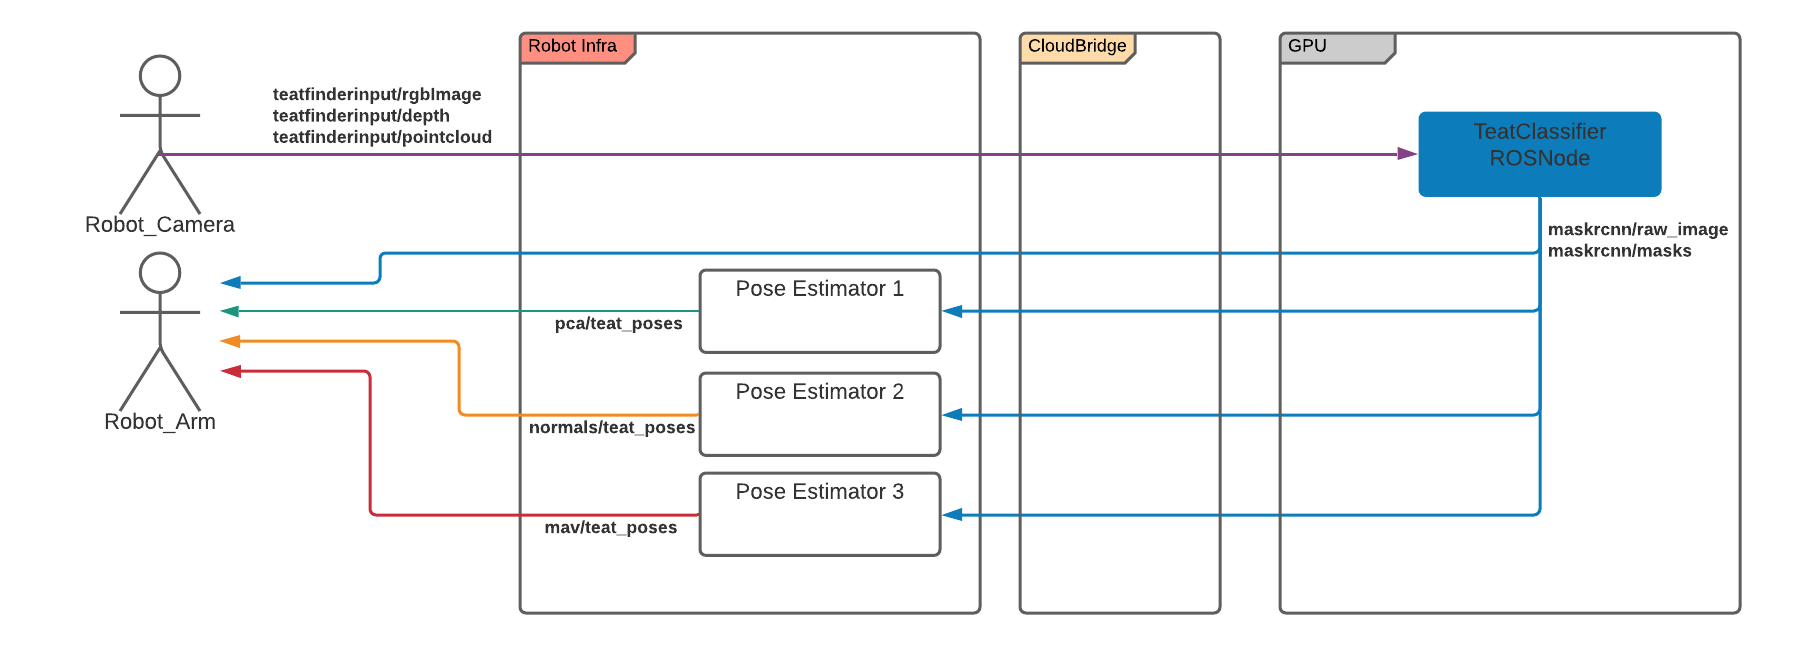
\includegraphics[width=1\textwidth]{images/cow_topics.png}
    \caption{A prototype of the Job Information dialog}
    \label{fig:cow_topics}
\end{figure}

\lipsum[2]\todo{TODO}. The described pipeline can also be represented visually as shown by Figure \ref{fig:cow_design}.
% The pose estimation algorithm was evaluated by error to GT
\begin{figure}[!ht]
    \centering
    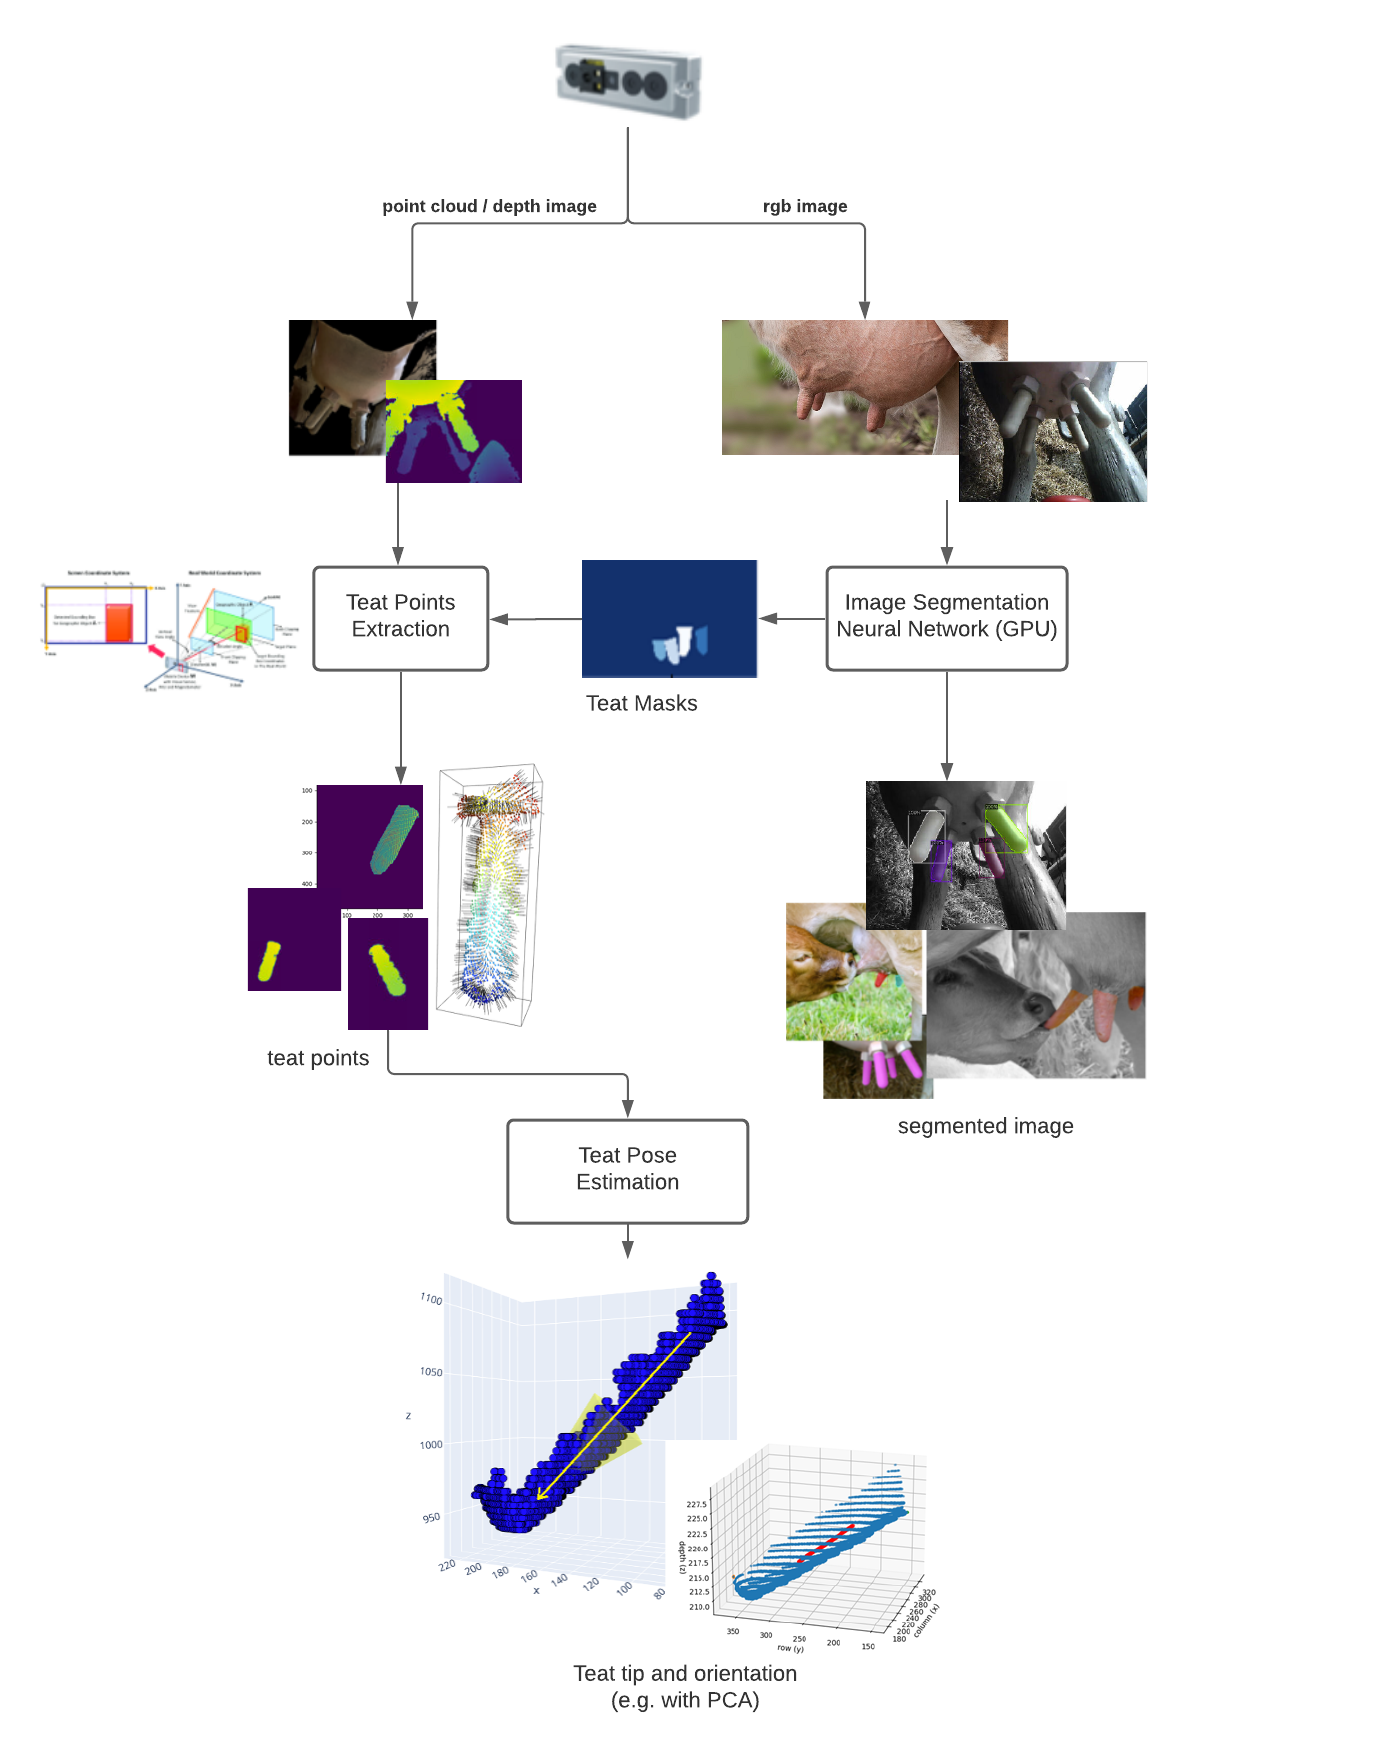
\includegraphics[width=0.9\textwidth]{images/cow_design.png}
    \caption{A prototype of the Job Information dialog}
    \label{fig:cow_design}
\end{figure}

% \begin{figure}[h]
%     \centering
%     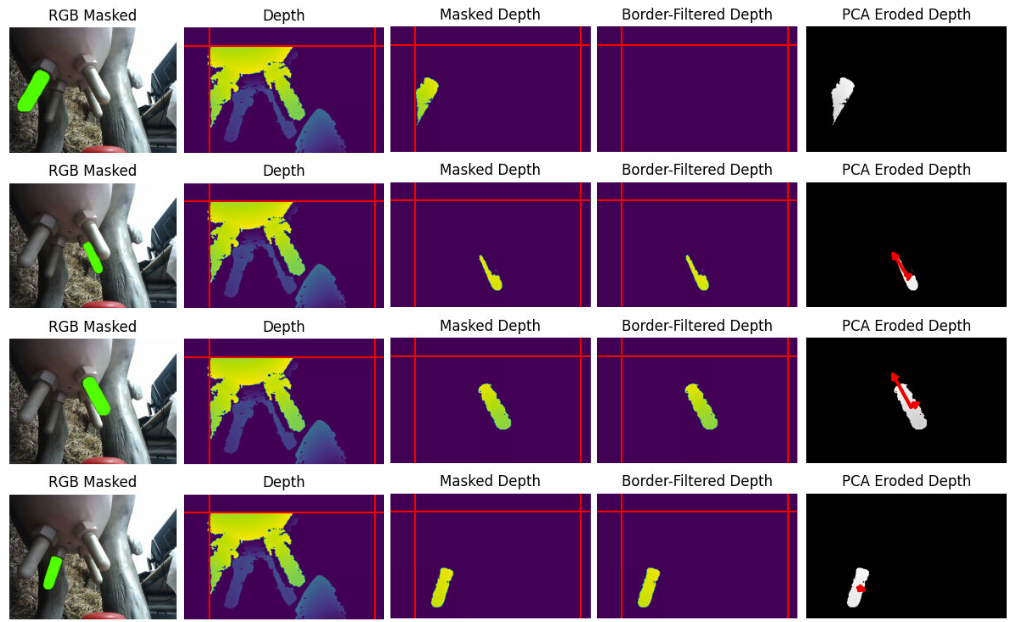
\includegraphics[width=0.6\textwidth]{images/cow_segment.png}
%     \caption{A prototype of the Job Information dialog}
%     \label{fig:cow_design}
% \end{figure}

% \begin{itemize}
%     \item rgb input, setup of the cow and angle of the camera 
%     \item networks architectures tried out: maskrcnn + pca, detectron + pca + subvariants
% \end{itemize}

For the deployment of the pipeline on the GPU servers, docker images were built per component (RViz, ROSPlay, ROSTeat, PoseEstimator, etc.). A set of docker compose files was used to control the deployment of the docker containers. Figure \ref{deploy:docker} shows a sample of a docker-compose file, which describes the services and the volumes being deployed.

\begin{figure}[h]
    \centering
    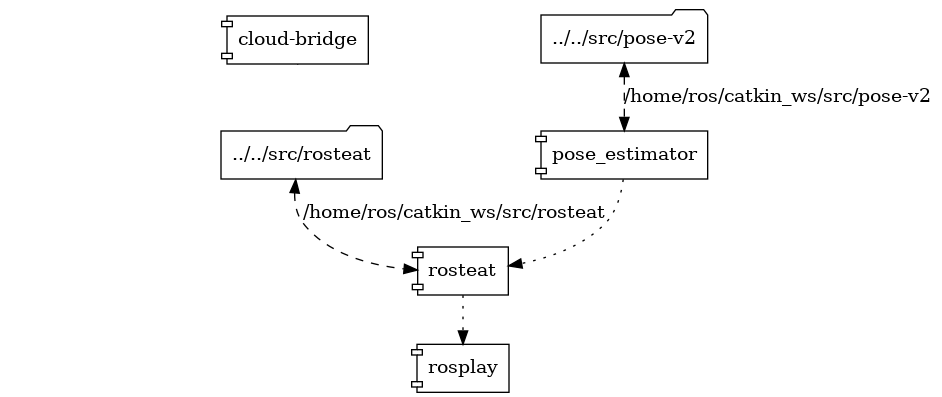
\includegraphics[width=0.6\textwidth]{images/cow_docker_topology.png}
    \caption{Image annotation example.}
    \label{fig:cow_docker_topology}
\end{figure}

% \lipsum[2-3]\todo{TODO}

\section{Training Data Collection}
The training data was collected using the robot's base recording procedure: the input images are stored as a video file in ROS format (ROSbag), which could be replayed for future testing or simulations. Once a ROSbag was stored, Rviz was used to collect RGB images and depth images at indicated timestamps (manual collection).

The collected images were then imported into LabelMe 
\ref{labelme}, where the pixel-wise segmentation areas were manually marked and the class label assigned. Figure \ref{fig:cow_labelme} shows a glimpse of the labelling process. Once an image has been labelled the pixel-wise segmentation is stored as a polygon in .json file next to the original image.

\begin{figure}[h]
    \centering
    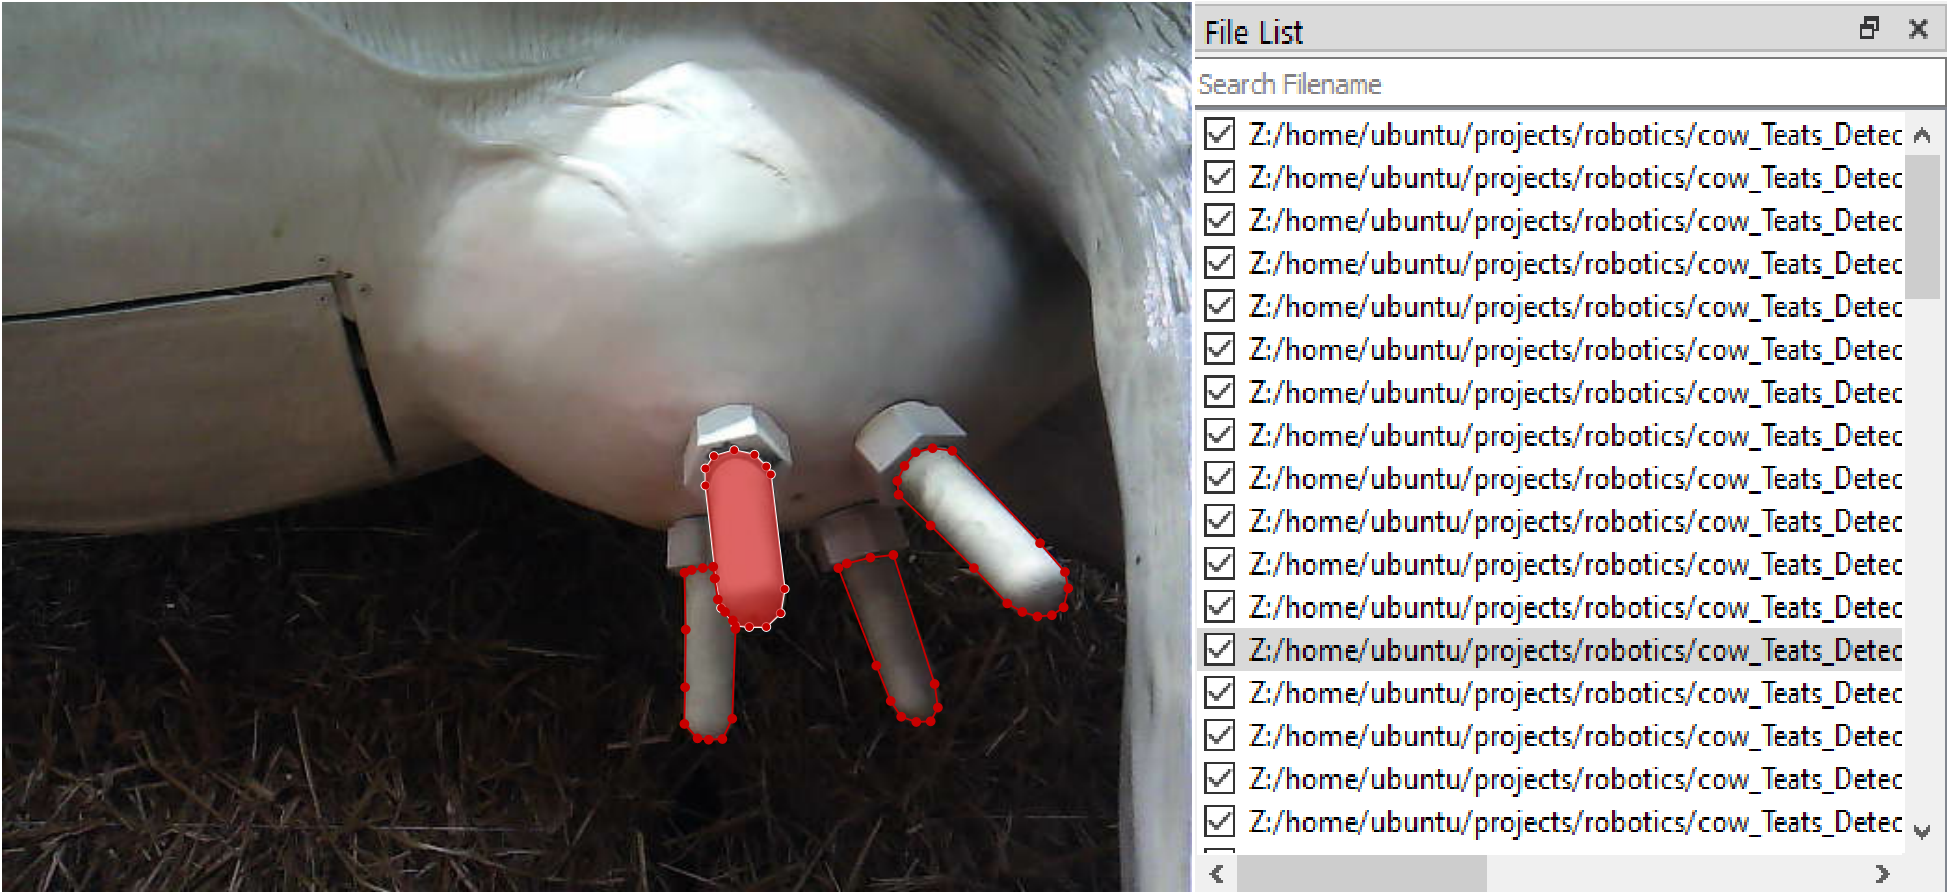
\includegraphics[width=0.6\textwidth]{images/cow_labelme.png}
    \caption{Image annotation example.}
    \label{fig:cow_labelme}
\end{figure}
    
% \begin{itemize}
%     \item 1 paragraph for describing the picture taking process from rosbags
%     \item 1 paragraph to describe how to label images, and then feed them to the detectron container
% \end{itemize}
We acknowledge that synthetic data does not reflect real camera data in regards of noise or different
lighting conditions. However we are confident that the approaches used can be transferred to real-world
data if sufficient labeled data (see discussion in section 5.4) are available, as has been shown in different
other publications [48, 49, 50].

For the generated scenes, we attempt to reach a visual level that includes many real-world properties
such as shadows, specular highlights, etc., but is still simple enough to make sure that potential
shortcomings of the algorithm cannot be accounted to scenes that are too complicated or to noisy.
We also include uniquely colored walls to enable the algorithm to internally assign global positions to
the objects (e.g. “The yellow cylinder is located towards the corner of the red and green wall”). Due
to time constraints, we do not evaluate the influence of these colored walls as part of this work but
leave this question open to follow-up research. To add additional variance to the input images, the
camera gets randomly rotated for each scene along the horizontal axis with an angle between +12.5
and −12.5
. As a consequence, this rotation needs to be considered when inferring positions of objects
or transforming stored object positions on frame changes.

\section{Neural Network Training}
All architectures are implemented in Python 3.7 and use PyTorch as machine learning framework
[51]. To train the system, we use a combination of 20, 000 scenes with and 20, 000 scenes without
occlusion. We let the system draw a random sample from this set for each batch. The used batch
size varies for each architecture and is determined by the memory requirements of the approach. For
the baseline version, we use 128, the CNN + RNN version uses 32 and the ConvLSTM version 64
elements per batch. The learning rate is the same for all approaches at 0.0001. We did not use any
form of hyperparameter search, but relied only on parameters that seemed to provide a stable training
performance with a few test runs. It can therefore be assumed that other parameter combinations exist
which would improve the training performance even further. All used network architectures are listed
in Appendix A

All training is performed on a NVIDIA Titan Xp Graphics Processing Unit (GPU) with 12 GB VRAM
and uses CUDA [52] to speed up the process.
The labelled images are used as input for a docker container which expects the following variables for training the classification network:
    \begin{itemize}
        \item TRAIN: 
        \item DATASET:
        \item 
        % \item 1 paragraph describe implementations, docker, etc
        % \item 1 paragraph describe the training hyperparameters for the networks
    \end{itemize}
A set of hyperparameters for the training of the network can be set, such as:
\begin{itemize}
    \item EPOCHS:
    \item THRESHOLD:
    \item LR:
\end{itemize}
% \section{Environment Setup}
% \begin{itemize}
%     \item how did we setup the environment (fake cow, training images, arm)
%     \item did we find some benchmark to compare to?
%     \item goal of system
% \end{itemize}

\section{Pipeline Evaluation}
We evaluate all networks on scenes with and without occlusion. For both setups, we use 1,000
test scenes each, which have never been seen on training time. We only list a subset of all stream
evaluations here. The evaluation of remaining streams can be found in the Appendix A. For evaluation
of the enumeration stream, we use the following metric (which we call success rate):

% S =
% #correctly identified
% #correctly identified + #incorrectly identified

As “correctly identified” we only count objects which are present in the scene with the matching color
and shape. As incorrectly classified objects we count objects which are duplicate, do not exist at all or
have not been found by the network. This is similar to accuracy, with the difference that the number of
correctly and incorrectly classified objects do not need to add up to the number of ground truth objects.
In the Table 3.1, we evaluate a subset of the streams presented in section 3.3 on the evaluation scenes
without occlusion.

As visible in Table 3.1, the CNN + RNN approach outperforms both the baseline and the ConvLSTM
version remarkably for all streams. While it could be assumed that the baseline would not perform
as well as CNN + RNN due to a lack of accumulating capability, the mediocre performance of the
ConvLSTM version is relatively surprising. We are unsure of the cause and cannot recognize a specific
pattern in which the ConvLSTM is under-performing. However, we assume that the fewer convolutional
layers before the ConvLSTM do not allow for such a good feature extraction as this is the case in the
CNN + RNN version. 
% This recurrent layer therefore needs to operate on less abstracted information,
% which could prove difficult. CNN + RNN on the other hand, does exceptionally well, and if it struggles,
% then mainly in cases where the two shapes “Cube” and “Cube-Hollow” are present, which do look
% similar by nature. The following Table 3.2 lists the results of evaluating scenes with occlusion.

An evaluation with fine tuning a pre-trained ResNet-18 as feature extractor did not lead to any
noticeable improvements. We assume that our scenes are generally too simple to actually use advantages
of such approaches. For more complex scenes, this needs to be re-evaluated.
    % \begin{itemize}
    %     \item 1 paragraph describe how we evaluated the algorithms: using the error from the teats on x y z
    %     \item 1 paragraph describe our interpretation of the results 
    %     \item describe how some other changes did not improve
    % \end{itemize}
% \section{VOID: Towards "better" Pose Estimation Algorithms}
%     \begin{itemize}
%         \item describe how a generic pose estimation algorithm should work/what we expect
%         \item describe something similar to 3d pose algorithm challenges and future work for generic SotA of 3d pose algorithms from related work
%     \end{itemize}
